\section{Example Domains}
We apply approximate abstraction to four example domains---NChain, Taxi, Minefield and Random. These domains were selected for their diversity---NChain is relatively simple, Taxi is goal-based and hierarchical in nature, Minefield is stochastic, and Random MDP has many near-optimal policies.

%Description of code base
Our code base\footnote{\url{github.com/david-abel/state_abstraction}} provides implementations for abstracting arbitrary \acp{MDP} as well as visualizing and evaluating the resulting abstract \acp{MDP}. We use the graph-visualization library GraphStream~\cite{graphstream} and the planning and \ac{RL} library, BURLAP\footnote{\url{http://burlap.cs.brown.edu/}}. For all experiments, we set $\gamma$ to $0.95$.

\subsection{Visualizations}

% Description of visuals.
We provide visuals of both the ground \ac{MDP} and resulting abstract \ac{MDP} for one domain. A grey circle indicates a state and colored arrows indicate transitions. The thickness of the arrow indicates how much reward is associated with that transition. In the ground \acp{MDP}, states are labeled with a number. In the abstract \acp{MDP}, we indicate which ground states were collapsed to each abstract state by labelling the abstract states with their ground states (some are visually unwieldy and so were not labelled).

% Subsection: NChain.
\subsubsection{NChain}

NChain is a simple \ac{MDP} investigated in the Bayesian \ac{RL} literature due to the interesting exploration problem it poses~\cite{dearden1998bayesian}. In our implementation, we set $N=10$, normalized rewards between $0$ and $1$, and used a slip probability of $0.2$.

In all states, the agent has two actions available: advance down the chain, or return to state 0. The agent receives $.2$ reward for returning to state 0, and no reward for advancing down the chain. The exception is that when the agent transitions to the last state in the chain, it receives $1.0$ reward. Transitions also have small slip probability $\rho$, such that the applied action results in the opposite dynamics. In our implementation, we set $N=10$ and $\rho=0.2$.
% NChain Compression Visuals.
\begin{figure}[h]
\centering
\subfigure[Ground NChain]{
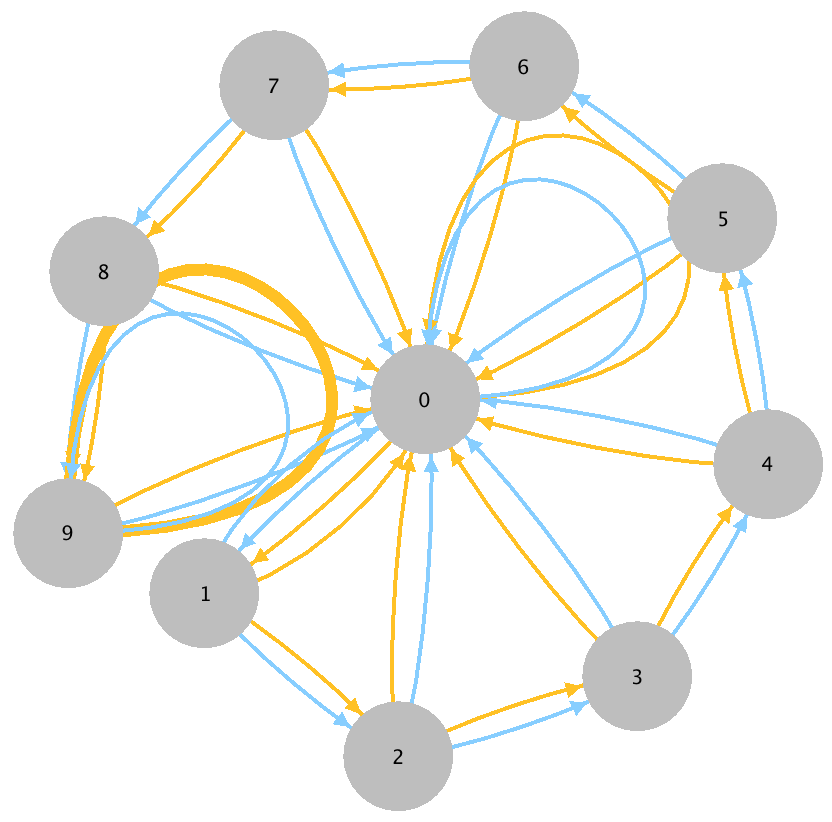
\includegraphics[width=0.20\columnwidth]{figures/ground_nchain_small.png}}
\hspace{6mm}
\subfigure[Abstract NChain]{
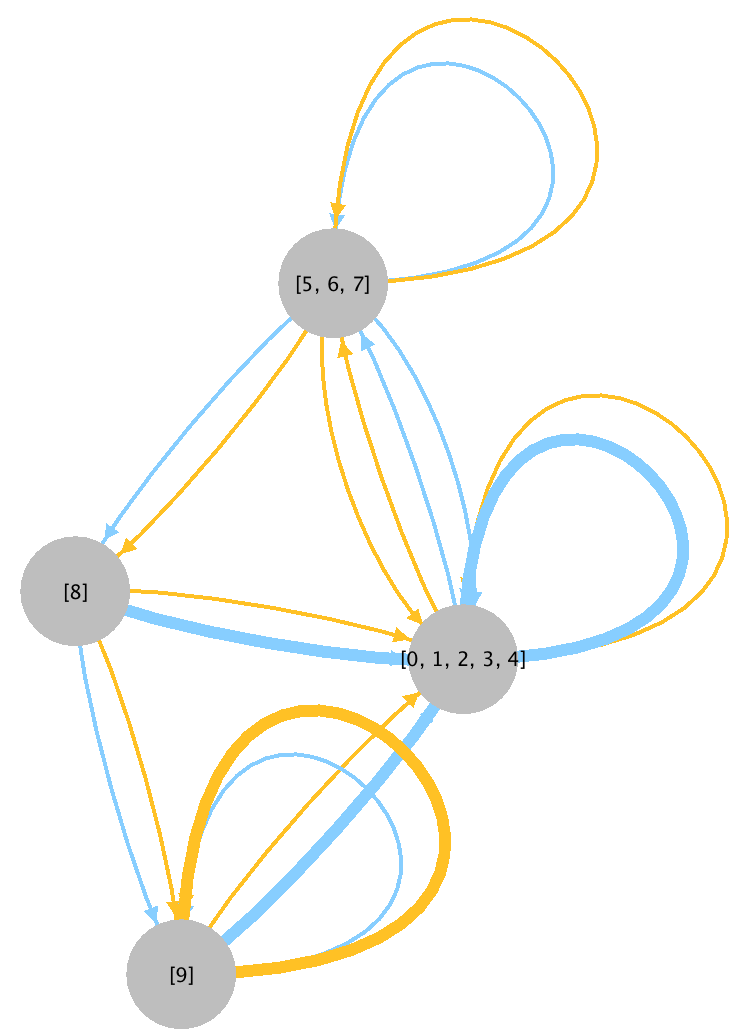
\includegraphics[width=0.20\columnwidth]{figures/abs_nchain.png}}
\label{fig:nchain-visual}
\caption{Comparison of ground NChain \ac{MDP} and abstract NChain \ac{MDP}, under an $\epQ$ abstraction, with $\varepsilon=0.5$}
\end{figure} 

% Subsection: UpWorld.
\subsubsection{UpWorld}

The UpWorld task is an $N\times M$ grid in which the agent starts in the lower left corner. The agent may move left, right, and up. The agent receives positive reward for transitioning to any state at the top of the grid, where moving up in the top cells self transitions. the agent receives 0 reward for all other transitions. Consequently, moving up is always the optimal action, since moving left and right does not change the agent's manhattan distance to positive reward. During experimentation, we set $N=10$, $M=4$.

As an aside, UpWorld illustrates a compelling property with respect to state abstraction: the optimal {\it exact} $Q^*$ abstraction function (when $\eps=0$) can always construct an abstract MDP with $|\mc{S}_A| = N$, the height of the grid, with no change in the value of the optimal policy. Consequently, letting $M$ be arbitrarily large, UpWorld offers an arbitrary reduction in the size of the MDP through abstraction, at no cost to the value of the optimal policy. More succinctly: \\

\noindent {\bf Remark}: {\it The optimal exact abstraction, $\phi_{Q^*,0}$, always induces an abstract MDP with an optimal policy of equal value to the true optimal policy. Further, $\phi_{Q^*,0}$ will reduce the size of the abstract state space from $N \times M$ to just $N$.} \\

This is a result of the property of UpWorld that all states in the same row will always have the same $Q$ value.
\begin{figure}[h]
\centering
\subfigure[Ground UpWorld]{
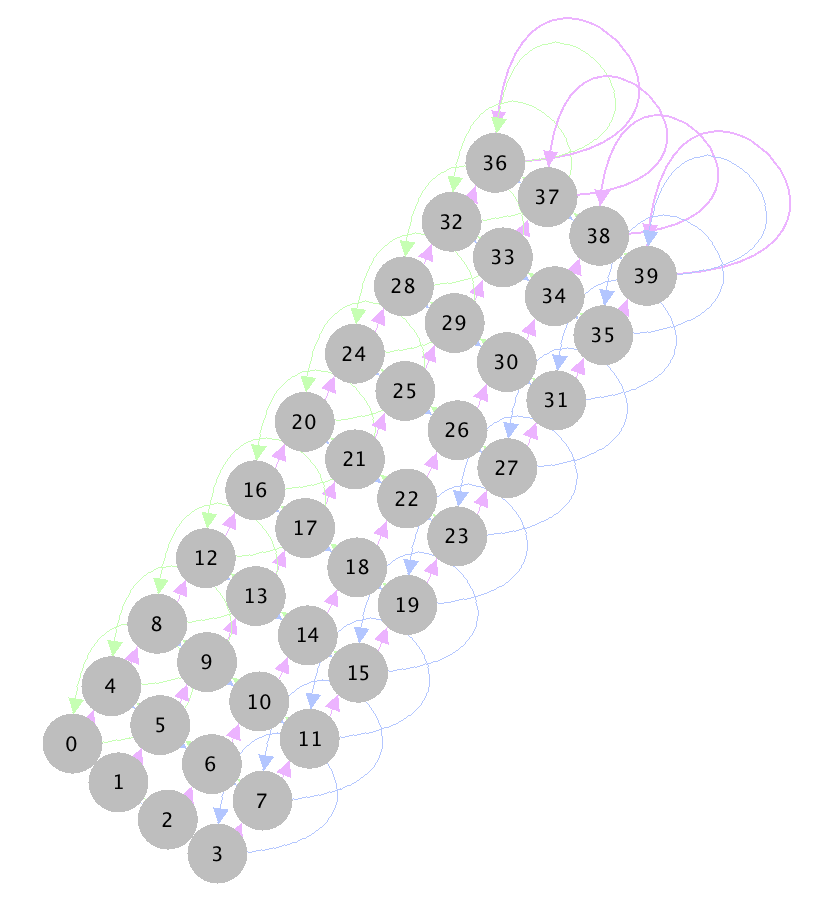
\includegraphics[width=0.25\columnwidth]{figures/ground_upworld.png}}
\hspace{6mm}
\subfigure[Abstract UpWorld]{
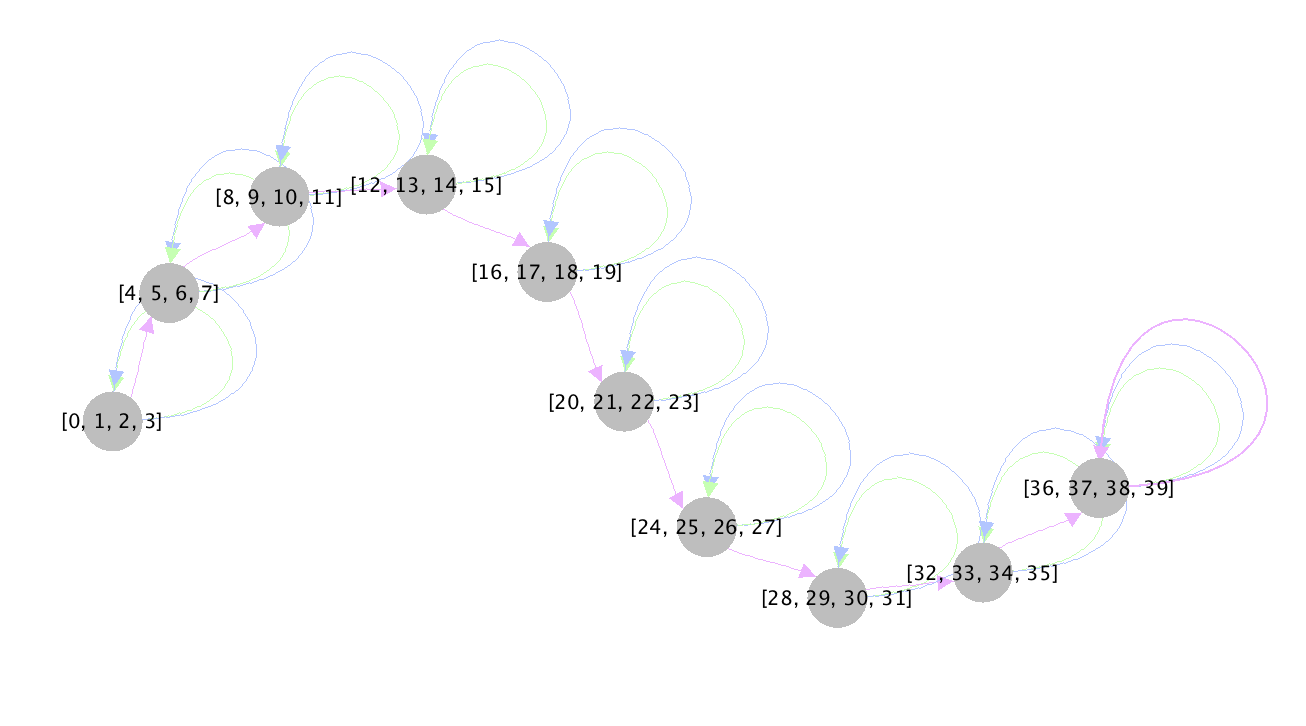
\includegraphics[width=0.14\columnwidth]{figures/abs_upworld.pdf}}
\label{fig:upworld-visual}
\caption{Comparison of Original UpWorld MDP and Abstract MDP, under $\epQ$, with $\varepsilon=0.5$}
\end{figure} 

% Subsection: Taxi
\subsubsection{Taxi}

Taxi has long been studied by the hierarchical RL literature~\cite{dietterich2000hierarchical}. The agent, operating in a Grid World style domain~\cite{russell1995modern}, may move left, right, up, and down, as well as pick up a passenger and drop off a passenger. The goal is achieved when the agent has taken all passengers to their destinations.

We visualize the compression on a simple 626 Taxi instance in Figure~\ref{fig:taxi-visual}. As stated above, we visualize the original Taxi problem into a graph representation so that we may visualize both the ground MDP and abstract MDP in the same format.

% Taxi Compression Visuals
\begin{figure}[h]
\centering
\subfigure[Ground Taxi]{
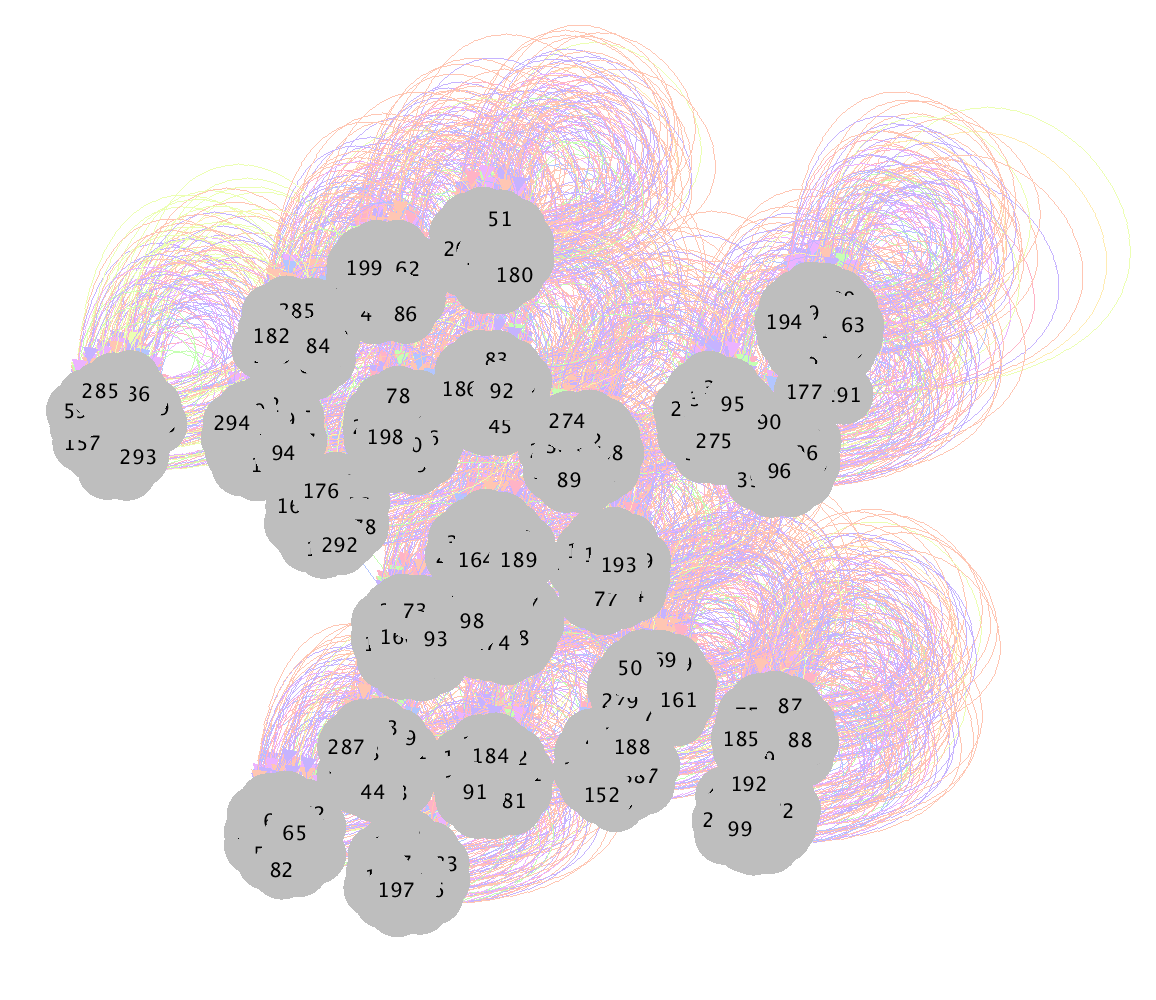
\includegraphics[width=0.25\columnwidth]{figures/ground_taxi.png}}
\hspace{6mm}
\subfigure[Abstract Taxi]{
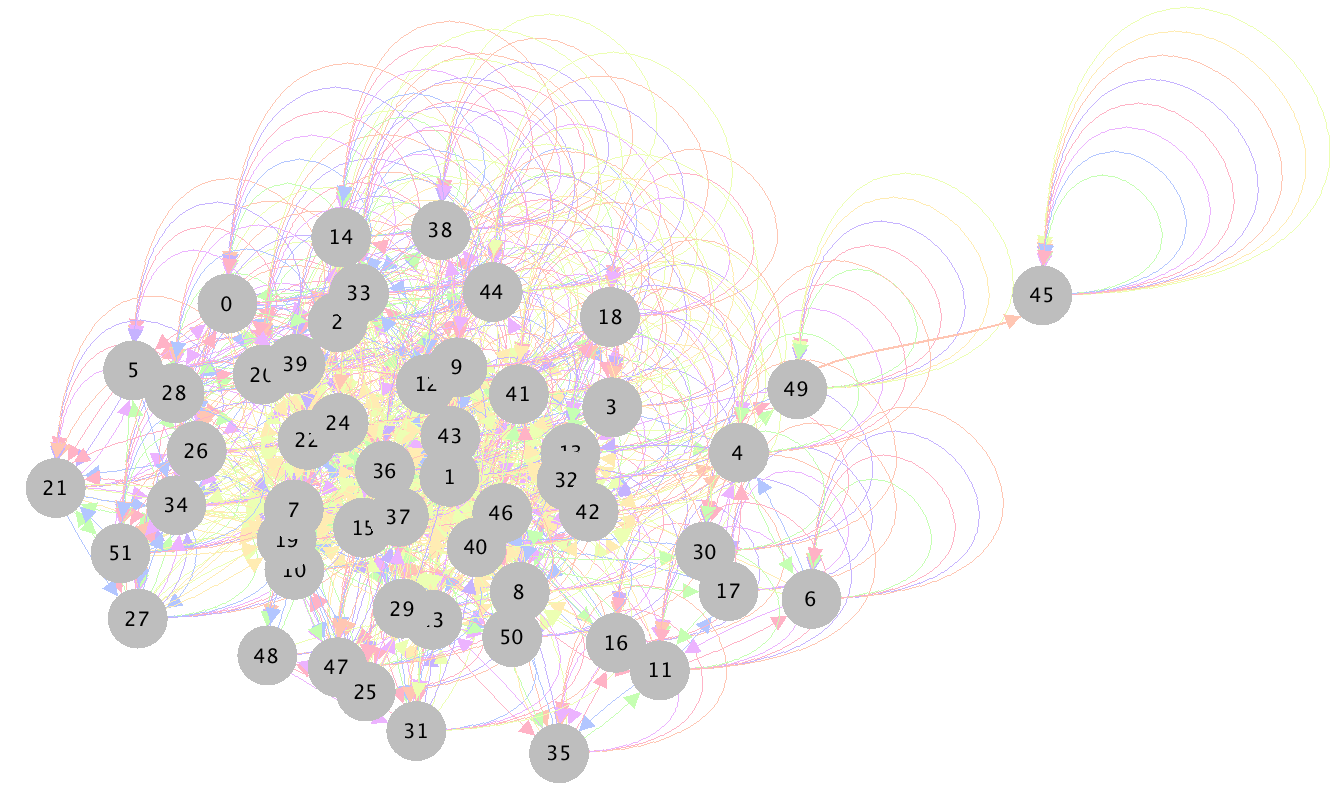
\includegraphics[width=0.25\columnwidth]{figures/abs_taxi.png}}
\label{fig:taxi-visual}
\caption{Comparison of Original Taxi MDP and Abstract Taxi MDP, under an $\epQ$ abstraction, with $\varepsilon=0.03$}
\end{figure} 


% Insert visual and/or stats on number of states and performance of VI solving the abstract MDP and evaluating the resulting policy on the original MDP


% Subsection: Minefield.
\subsubsection{Minefield}
Minefield is a test problem we are introducing that uses the Grid World dynamics of \citet{russell1995modern} with slip probability of $x$. The reward function is such that moving up in the top row of the grid receives $1.0$ reward; all other transitions receive $0.2$ reward, except for transitions to a random set of $\kappa$ states (which may include the top row) that receive $0$ reward. (These are the states with ``mines'' in them.) We set $N=10, M=4, \varepsilon=0.5, \kappa = 5, x = 0.01$.
% Minefield Compression Visuals
\begin{figure}[h]
\centering
\subfigure[Ground Minefield]{
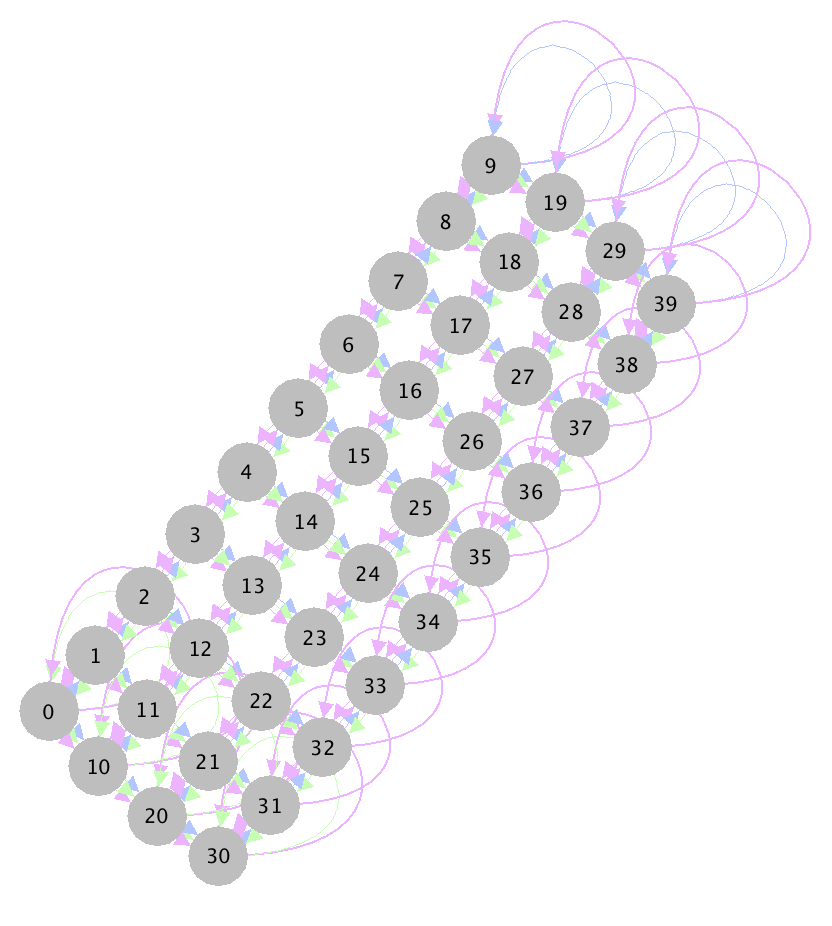
\includegraphics[width=0.15\columnwidth]{figures/ground_minefield.png}}
\hspace{6mm}
\subfigure[Abstract Minefield]{
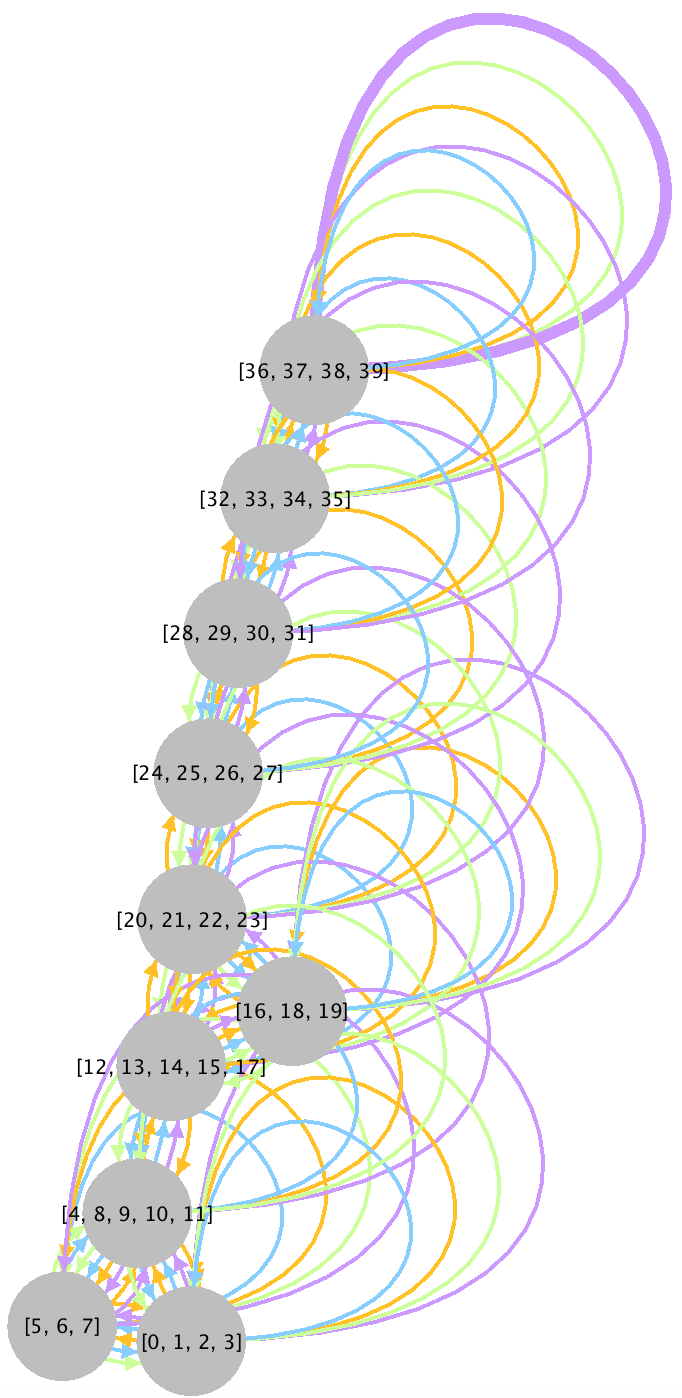
\includegraphics[width=0.15\columnwidth]{figures/abs_minefield.png}}
\caption{Comparison of ground Minefield \ac{MDP} and abstract \ac{MDP}, under a $\epQ$ abstraction with $
\varepsilon=0.5$}
\label{fig:minefield-vis}
\end{figure} 
 Subsection: Random.
\subsection{Random}
In the Random \ac{MDP} domain we consider, there are $100$ states and $3$ actions. For each state, each action transitions to one of two randomly selected states with probability $0.5$. The Random MDP and its compression are visualized in Figure~\ref{fig:minefield-visual}.

% Random Compression Visuals
\begin{figure}[h]
\centering
\subfigure[Ground Random]{
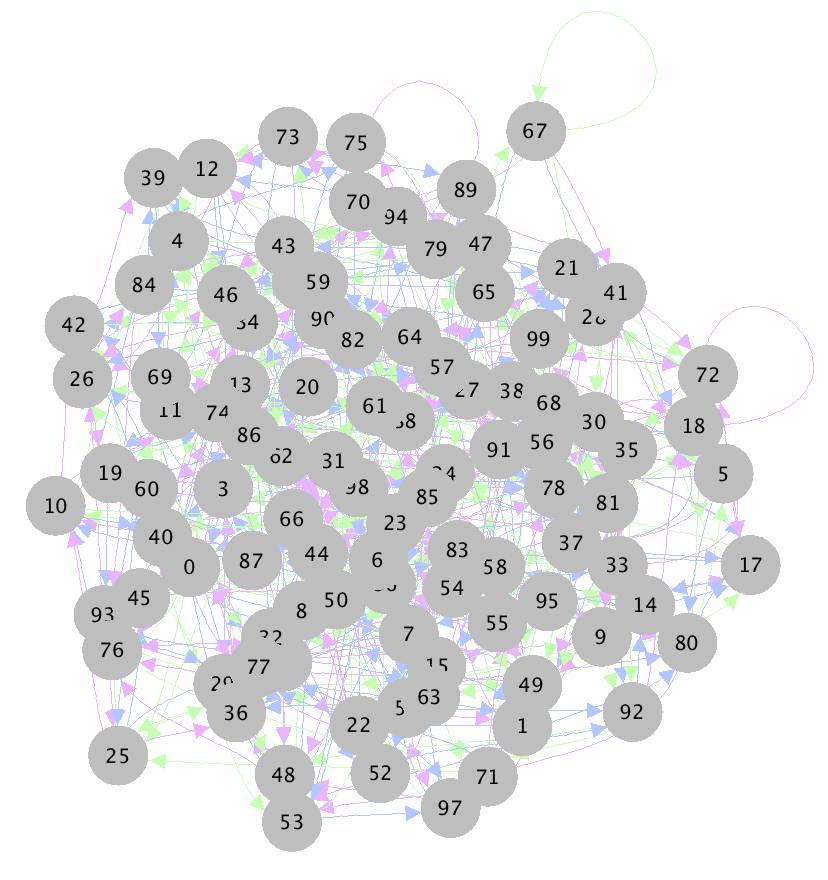
\includegraphics[width=0.25\columnwidth]{figures/ground_random.png}}
\hspace{6mm}
\subfigure[Abstract Random]{
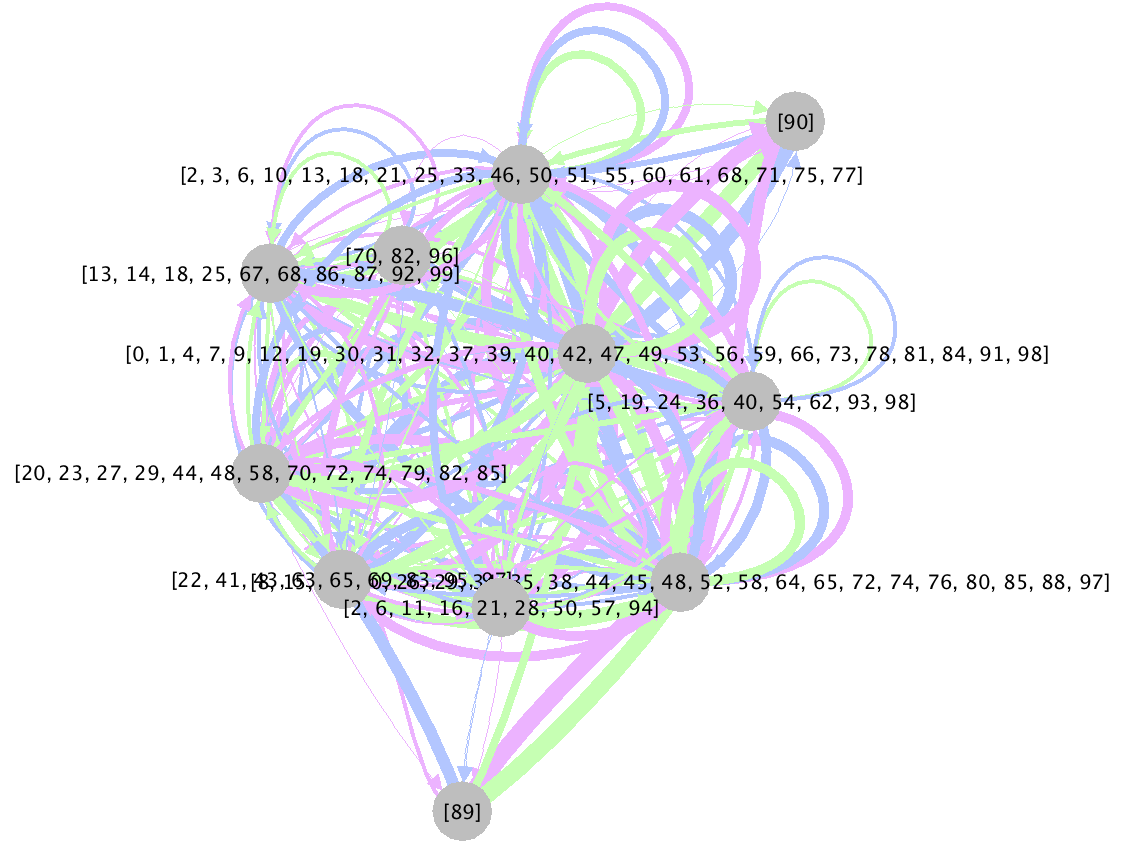
\includegraphics[width=0.25\columnwidth]{figures/abs_random.png}}
\label{fig:minefield-visual}
\caption{Comparison of Original Random MDP and Abstract Random MDP, under an $\epQ$ abstraction, with $\varepsilon=0.2$}
\end{figure} 
